\documentclass[twocolumn, a4paper, uplatex]{UECIEresume}

\usepackage[dvipdfmx]{graphicx}
\usepackage{graphicx}
\usepackage{amsmath}
\usepackage{txfonts}
\usepackage{array}
\usepackage{url}

\title{自然言語処理によるフェイクニュース判断の自動化}
\date{平成 30 年 9 月 25 日}
\affiliation{総合情報学科 メディア情報学 コース}
\supervisor{大須賀 昭彦 教授, 田原 康之 准教授, 清 雄一 准教授}
\studentid{1510151}
\author{栁 裕太}
\headtitle{平成 30 年度 総合情報学科 卒業論文中間発表}
%\headtitle{平成 yy 年度 総合情報学科 卒業論文発表}
%\headtitle{平成 yy 年度 総合情報学科 修士論文中間発表}
%\headtitle{平成 yy 年度 総合情報学科 修士論文発表}

\begin{document}
\maketitle

\section{背景}
インターネット環境の浸透により、フェイクニュースの急速な拡散が大きな社会問題として近年取り沙汰されている。
主に人々の扇動を目的に作られたフェイクニュースは、受け手に専門知識がない場合判断が難しい。
そこで有識者が発信された情報の信頼性を判断・公表するファクトチェックが主に米国で盛んになっている状況である。
しかしながら新たに発信される情報とファクトチェックには時間差があり、その間に拡散されてしまう状況となっている。
そこで過去のファクトチェック結果による機械学習モデルを構築することで、
新たに発信されるフェイクニュースに対応することを考えた。

今回の実験には、発言引用と真偽の要素を併せ持つデータセットが必要である。
使用したのは、ファクトチェック機関politifact.comのファクトチェック結果からなる
LIAR datasetを使用した\cite{pants}。
LIAR dataset掲載の真偽データはpolitifact.comの評価方法"Truth-O-Meter"に準拠しており、
真偽の度合いによって"Truth"〜"Pants-on-Fire"までの7段階評価となっている\cite{truth}。

今回の実験では、自然言語処理によってどれだけ正確に信頼性を自動で判定することができるか調べたものとなっている。

\section{課題}
課題として挙げられるのは、以下の2点である。
\begin{itemize}
  \item ファクトチェック機関によって蓄積された結果と、新型機械学習手法との親和性が不明である点
  \item 新たなニュースとファクトチェック結果が出るまで時間差がある点
\end{itemize}
特に後者では、ファクトチェック機関の調査が終わるまで少々の時間差があるため、
ファクトチェック結果が公表されても浸透しないというケースが起こりやすい。
そこで、その時間差を信頼性を自動算出・公表することで、
フェイクニュースの拡散に足止めを行うことを考えた。

\section{アプローチ}
今回扱う課題を解決するためには、以下のアプローチが必要である。
\begin{itemize}
  \item 最新の自然言語処理技術によってファクトチェックを自動化する
  \item 自動ファクトチェックシステムをSNS上へ適用する
\end{itemize}


\section{現在の進捗}
前者のアプローチに関して、実際に予備実験を行った。
全体の流れとしては、以下の図\ref{fig:nagare}の通りである。

\begin{figure}[h]
  \begin{center}
    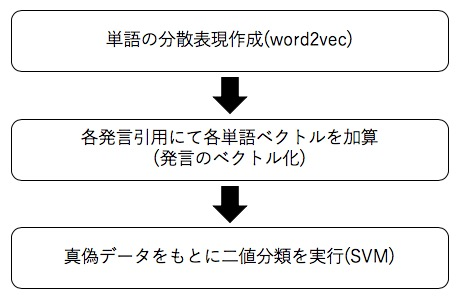
\includegraphics[width=8cm]{fig1.jpg}
    \caption{予備実験の流れ図}
    \label{fig:nagare}
  \end{center}
\end{figure}

まずは全体データセットの発言引用を元にword2vecによる単語の分散表現を作成する。
その次に各発言内にて、発言がもつ各単語ベクトルを加算・正規化することで、発言のベクトル化を行う。
最後に、各発言ベクトルと真偽を元にSVMで教師あり学習・検証を実行する。

LIARデータセットの真偽値に関しては、"Pants-on-Fire"〜"Mostly-False"をFalse、
"Half-True"〜"True"をTrueとして扱った。
なお、その場合の全体件数はTrueはXXXX件, FalseはXXXX件だった。

5分割交差検定を行った結果が以下の表\ref{tb:result}の通りである。

\begin{table}[h]
  \begin{center}
    \caption{予備実験結果}
    \label{tb:result}
    \begin{tabular}{c c}
      \hline
      データ名 & 数値 \\
      \hline \hline
      Precision & 0.723439 \\
      Recall & 1.000000 \\
      F1 score & 0.839530 \\
      \hline
    \end{tabular}
  \end{center}
\end{table}

Precision(適合率)は全体でのモデルの正答率、
Recall(再現率)はTrue全体内でのTrue看破率を表し、
F1 score(F値)は上記2値の調和平均を表す。

この結果より、word2vec+SVMの手法は良好な分類成績を示すことが判明した。

\section{今後の展望}
今後は、このフェイクニュース検出システムを実際のSNS上で運用する場合を想定したモデル作りが必要である。
そのために必要なものは、対象となる情報を選定することと、検証方法を考案する必要がある。

また、今回扱ったデータセットは全て英語・米国における情報だった。
もしもこれを日本語で運用することを考えた場合、
日本語でLIAR datasetとほぼ同じ情報形式を持つデータセットが必要である。
そのためには日本における第三者機関によるファクトチェックの活発化が求められるが、
残念ながらそのような運動があまりみられないのが現状である。

また,引用文献はキチンと入れましょう\cite{Kinoshita1}.引用は,先人に対するリスペクトなので,よほど独立性が高い研究でない限り必要となります.

{\small
\begin{thebibliography}{*}
  \bibitem{pants}Wang, William Yang. \textit{"liar, liar pants on fire": A new benchmark dataset for fake news detection}. Proceedings of the 55th Annual Meeting of the Association for Computational Linguistics (Volume 2: Short Papers)(2017):422-426.
  \bibitem{truth}Angie Drobnic Holan. \textit{The Principles of the Truth-O-Meter: PolitiFact’s methodology for independent fact-checking}. \url{https://www.politifact.com/truth-o-meter/article/2018/feb/12/principles-truth-o-meter-politifacts-methodology-i/}. (Sep. 18, 2018).
\end{thebibliography}
}
\end{document}
